\chapter{SIMULATION}\label{chap-simulation}
\thispagestyle{empty}

In this chapter, the design and performance of the UCC21330 gate driver in both half-bridge and full-bridge configurations are simulated and analyzed. The simulations are conducted to validate the circuit design, evaluate switching performance, and ensure correct operation under expected load conditions.

\section{Half-Bridge Driver Simulation}
The half-bridge circuit simulation diagram, shown in Figure~\ref{fig:halfbridge-sche}, forms the basic building block for driving power devices in switching applications.To validate the theoretical design, a SPICE-based simulation was conducted in TINA software. The simulation parameters were configured to match the component specifications found in the respective datasheets. The UCC21330 driver is employed to provide isolated, high-speed gate control with robust protection features.

\vspace{10pt}

The simulation results of the half-bridge circuit are presented in Figure~\ref{fig:halfbridge-result}. $V_\text{ds1}$ and $V_\text{ds2}$ are the drain source voltage across $S_\text{1}$ and $S_\text{2}$ respectively. $V_\text{gs1}$ and $V_\text{gs2}$ are the gate source voltage across $S_\text{1}$ and $S_\text{2}$ respectively.
\\[8pt]
The results confirm the proper switching action of UCC21330 gate driver at the required switching frequency of 100 kHz, voltage waveforms, and the timing characteristics of the driver. This validation ensures that the driver can handle the intended load and the switching frequency reliably.


\begin{figure}[H]
\centering
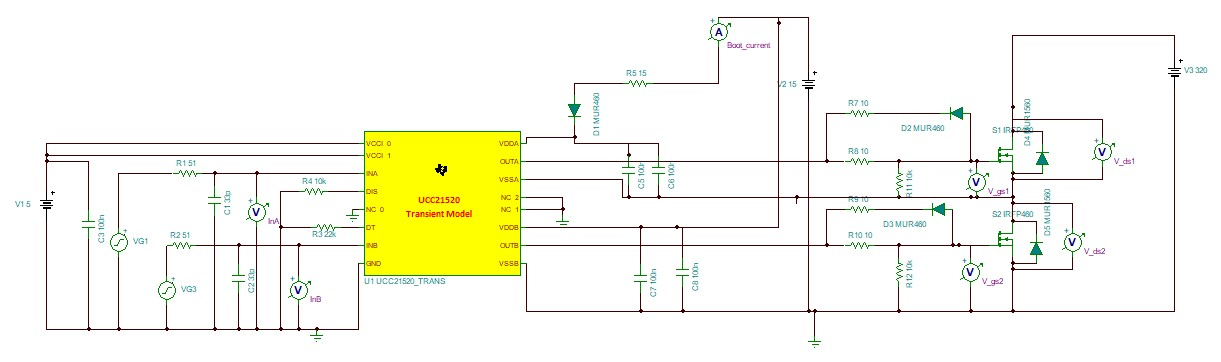
\includegraphics[width=1.5\linewidth, angle=90]{./picture-files/ucchalf.JPG}
\caption[Half-Bridge Driver Schematic]{Schematic of the half-bridge circuit using the UCC21330 gate driver.}
\label{fig:halfbridge-sche}
\end{figure}
\vspace{8pt}

\begin{figure}[H]
\centering
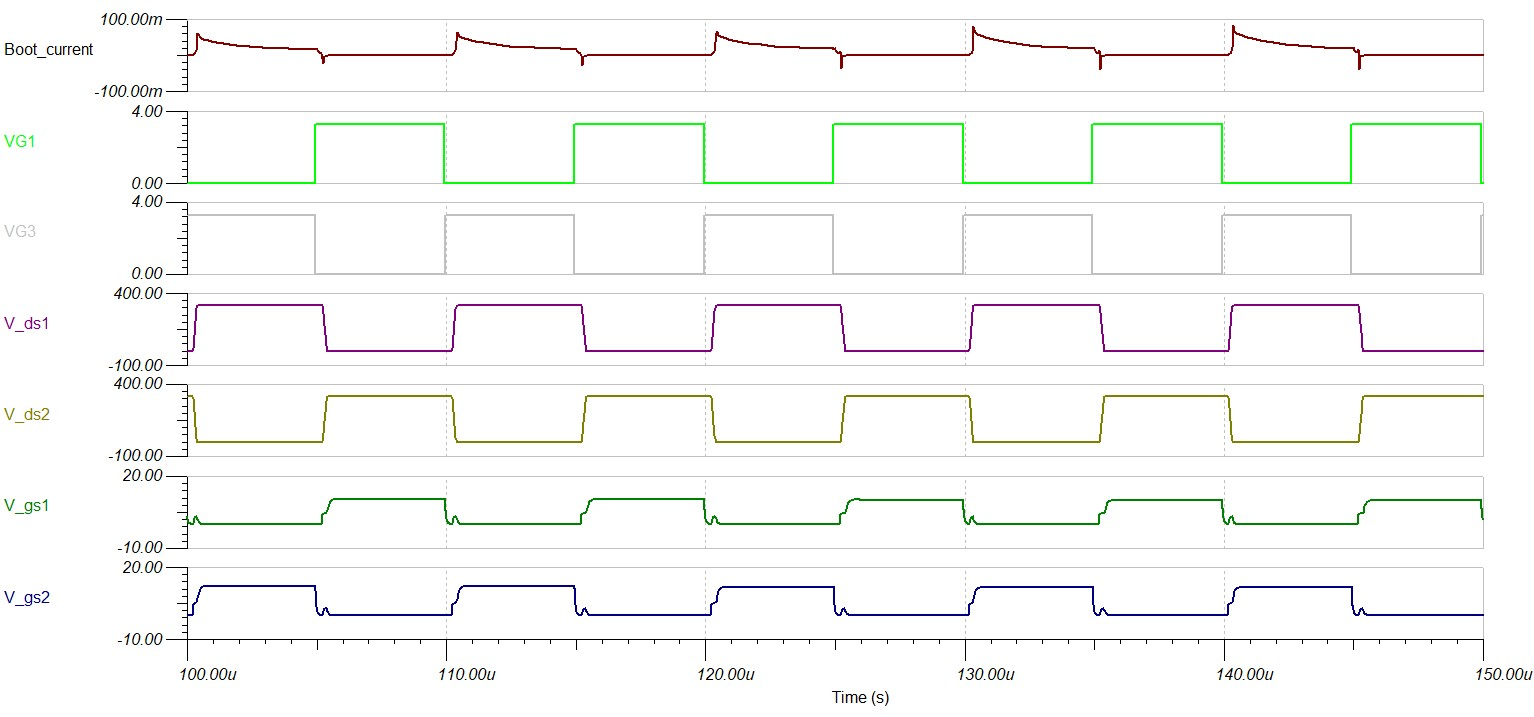
\includegraphics[width=1.5\linewidth, angle=90]{./picture-files/uccsimul.jpg}
\caption[Half-Bridge Simulation Result]{Simulation results of the half-bridge circuit using the UCC21330 driver.}
\label{fig:halfbridge-result}
\end{figure}

\section{Full-Bridge Driver Simulation}
The full-bridge configuration extends the half-bridge design. This simulation is also done in TINA-TI software. The simulation was done to validate the switching logic and output characteristics before proceeding to the hardware implementation. This simulation ensures that the gate signals are correctly timed to prevent shoot-through currents and confirms that a stable, symmetrical AC waveform is delivered to the high-frequency transformer primary. 
\\[8pt]The full--bridge schematic is shown in Figure~\ref{fig:fullbridge-sche}.
$V_\text{gs1}$, $V_\text{gs2}$, $V_\text{gs3}$ and $V_\text{gs4}$ are the gate source voltage across $S_\text{1}$, $S_\text{2}$, $S_\text{3}$ and $S_\text{4}$ respectively. The output voltage is also shown for a DC input of 320V.
\\[8pt] From the simulation it is observed that there might be a possibility of occurence of miller effect between gate and source voltage of the MOSFETs. This might end up in false turn on of MOSFETs therefore preventive steps were taken in the later stage.

\begin{figure}[H]
\centering
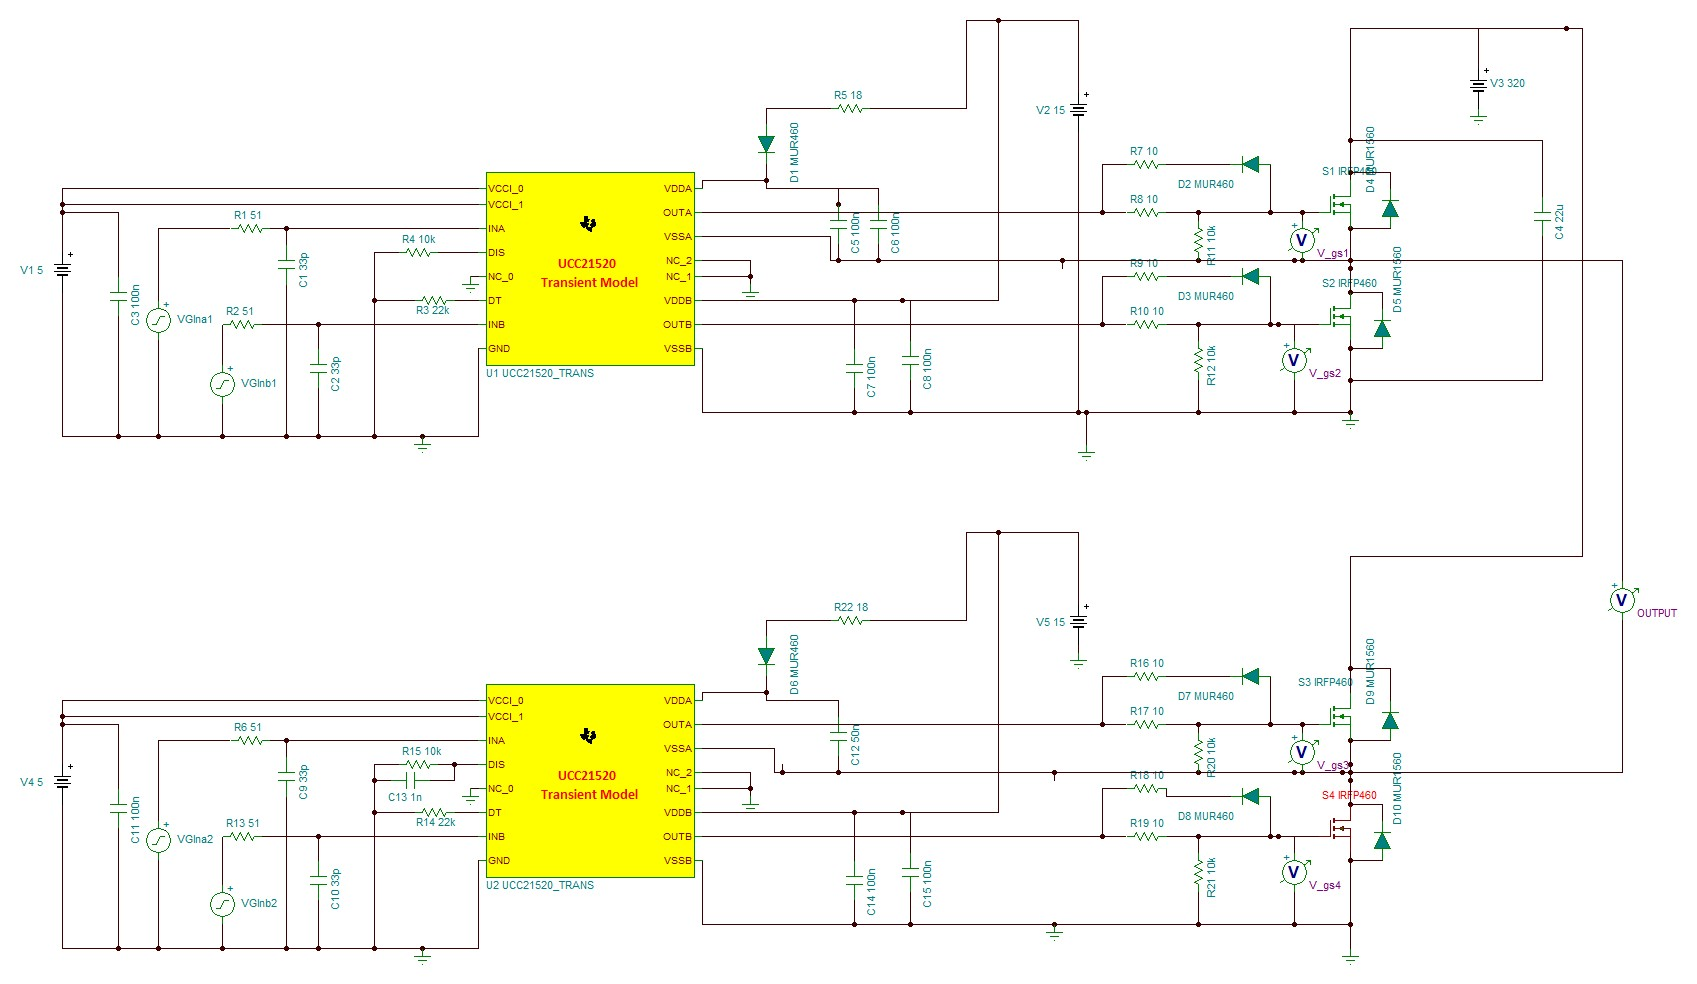
\includegraphics[width=1.5\linewidth, angle=90]{./picture-files/uccfull.JPG}
\caption[Full-Bridge Driver Schematic]{Schematic of the full-bridge circuit using the UCC21330 gate driver.}
\label{fig:fullbridge-sche}
\end{figure}


\begin{figure}[H]
\centering
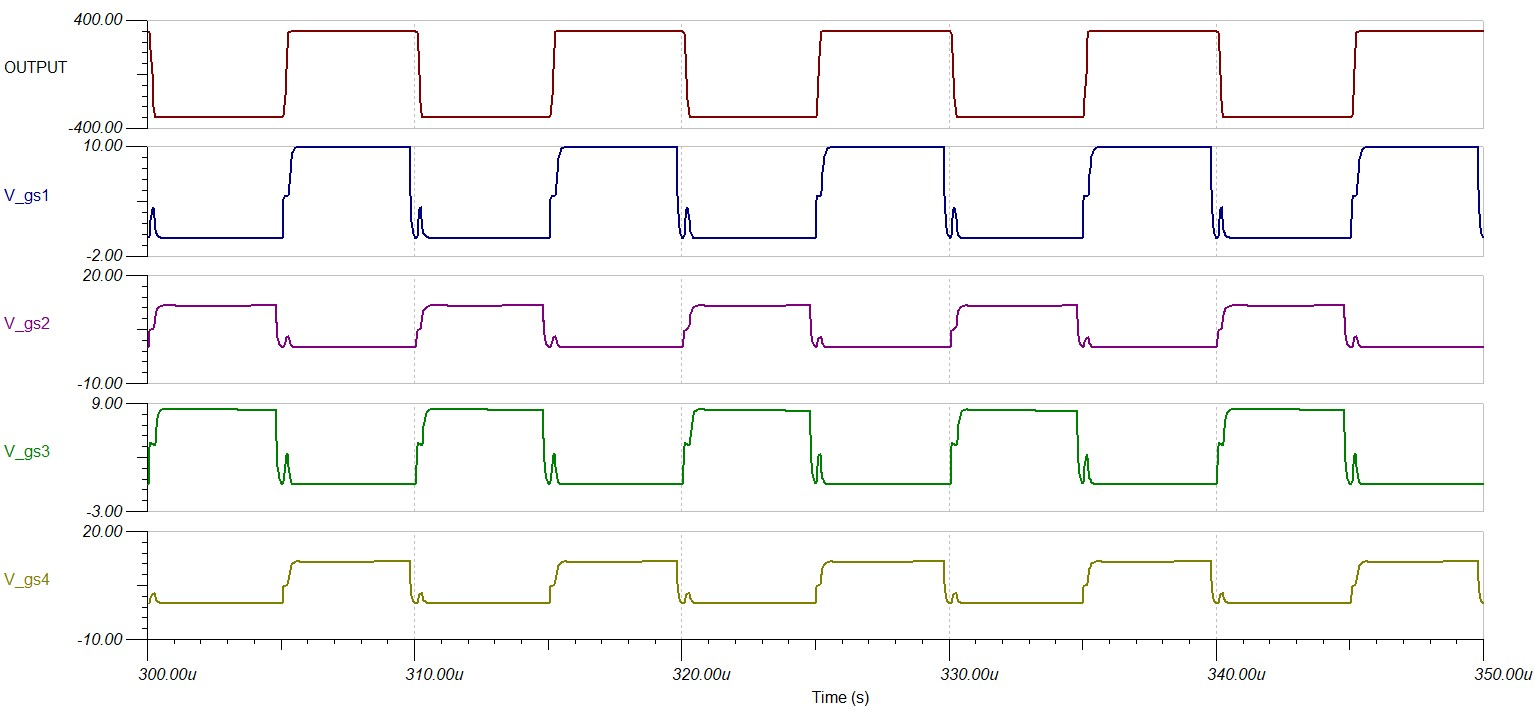
\includegraphics[width=1.1\linewidth]{./picture-files/fullresult.jpg}
\caption[Full-Bridge Simulation Result]{Simulation results of the full-bridge circuit using the UCC21330 driver.}
\label{fig:fullbridge-result}
\end{figure}


\section{Transformer Simulation}

\begin{figure}[H]
\centering
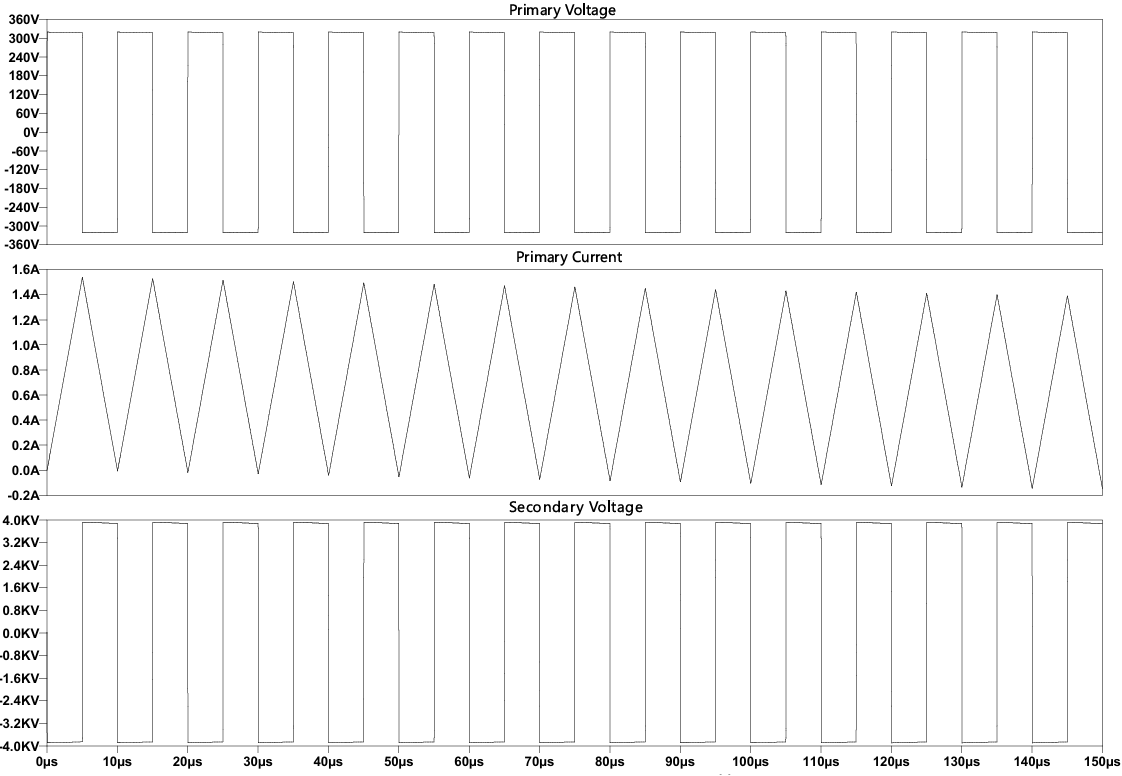
\includegraphics[width=1.1\linewidth]{./picture-files/transformersimulation.png}
\caption[Transformer Simulation Result]{Simulation result of the transformer in open circuit.}
\label{fig:transformer-result1}
\end{figure}

\begin{figure}[H]
\centering
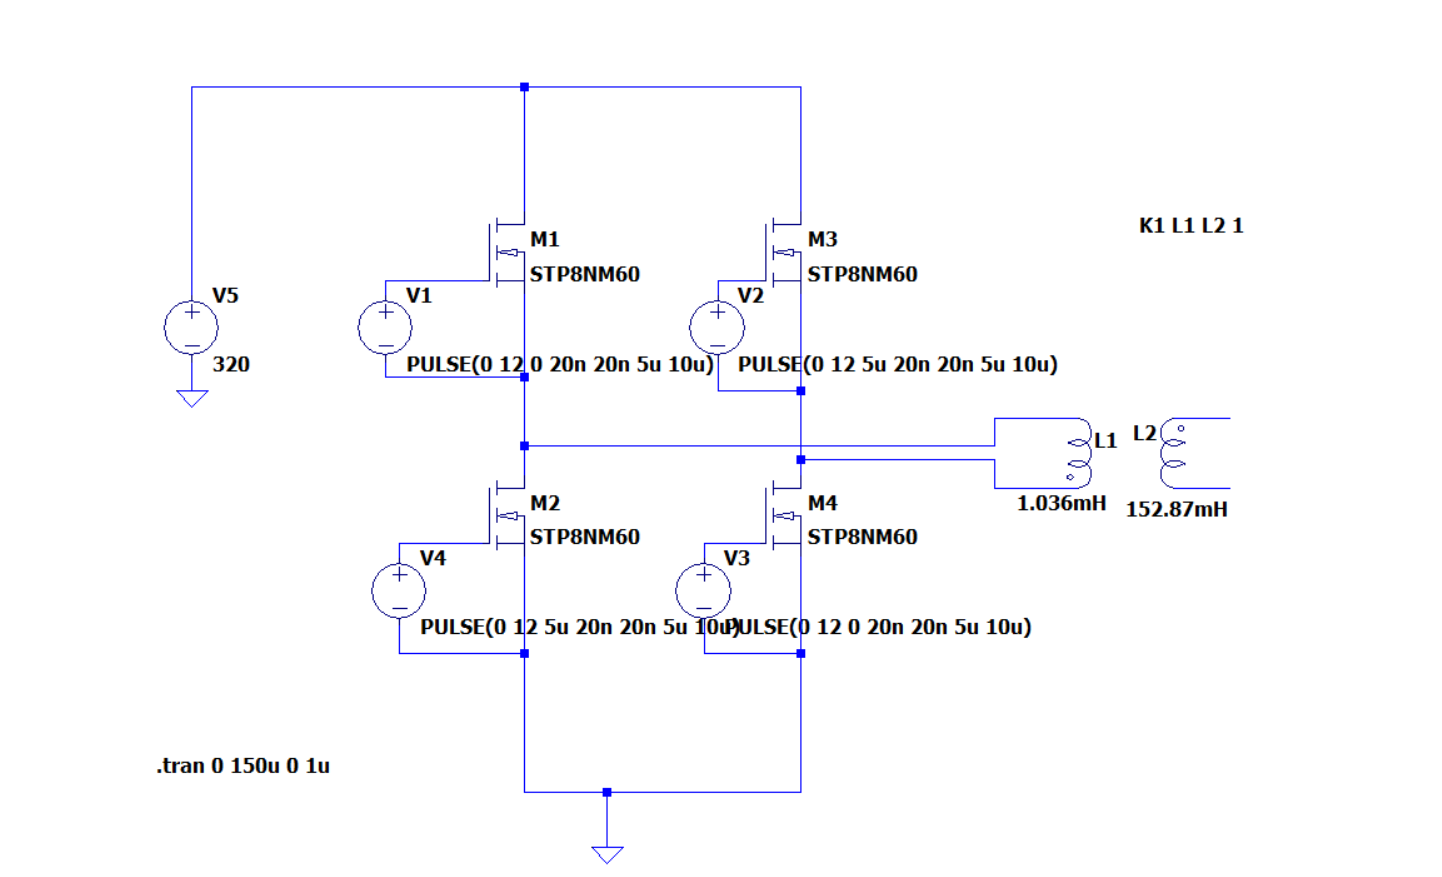
\includegraphics[width=1.1\linewidth]{./picture-files/transformercircuitsimul.png}
\caption[Transformer Simulation Result]{Simulation circuit of the transformer in open circuit.}
\label{fig:transformsimcir}
\end{figure}

\section{Cockroft - Walton Simulation}
The simulation of 4 stage Cockroft-Walton multiplier was done in LTSpice to determine the approximate output voltage from the input. In the simulation it was observed that after $38.6 kV$. The simulation output is shown in figure \ref{fig:simucockroft}
\begin{figure}[H]\centering

{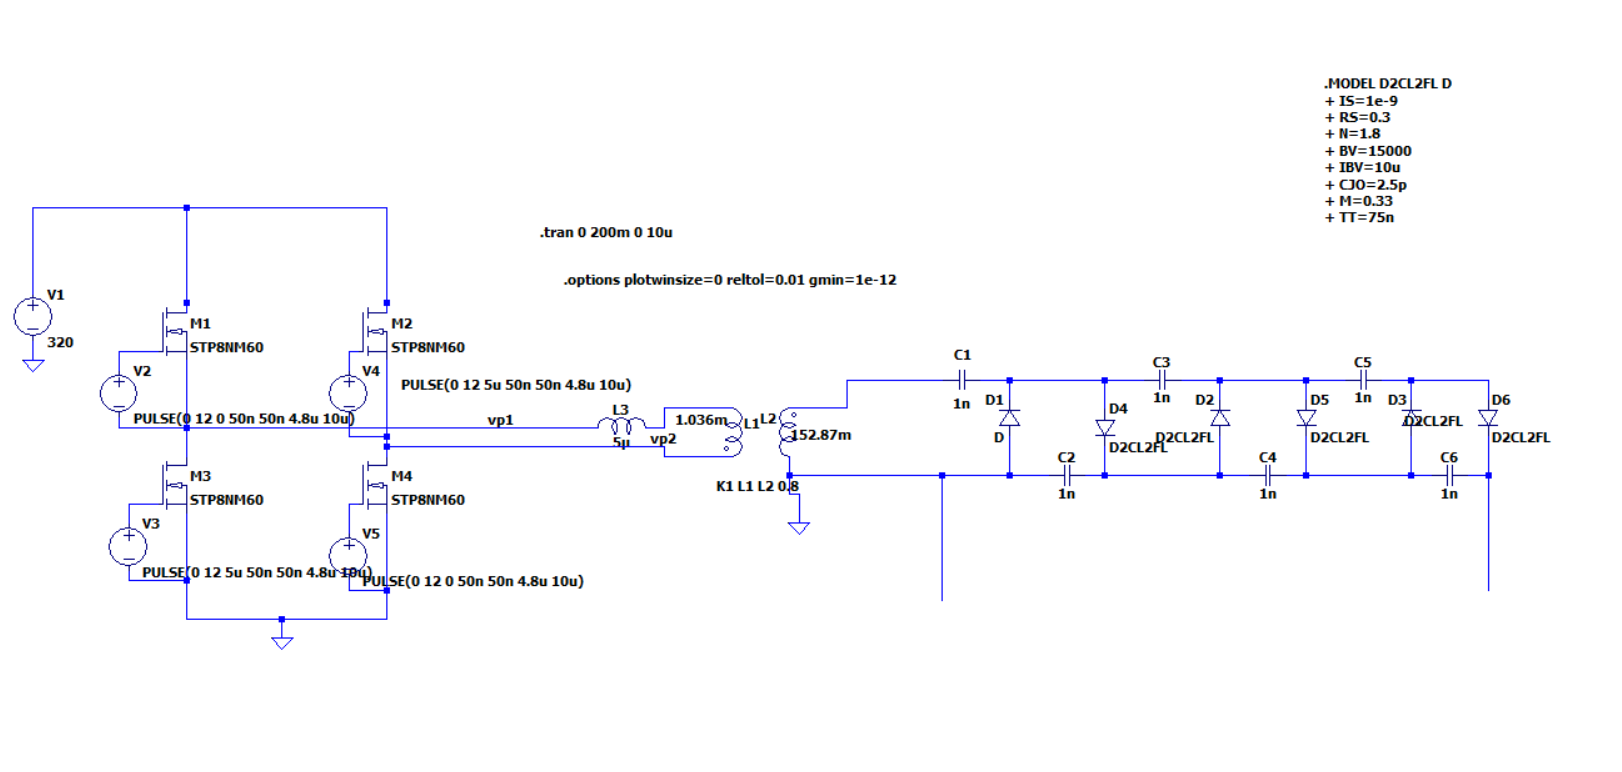
\includegraphics[width=1\textwidth]{./picture-files/cockcircuit.png}}
 \caption{Simulation circuit of cockroft walton multiplier}
    \label{fig:simucockroft}
\end{figure}\hfill

\begin{figure}[H]\centering
{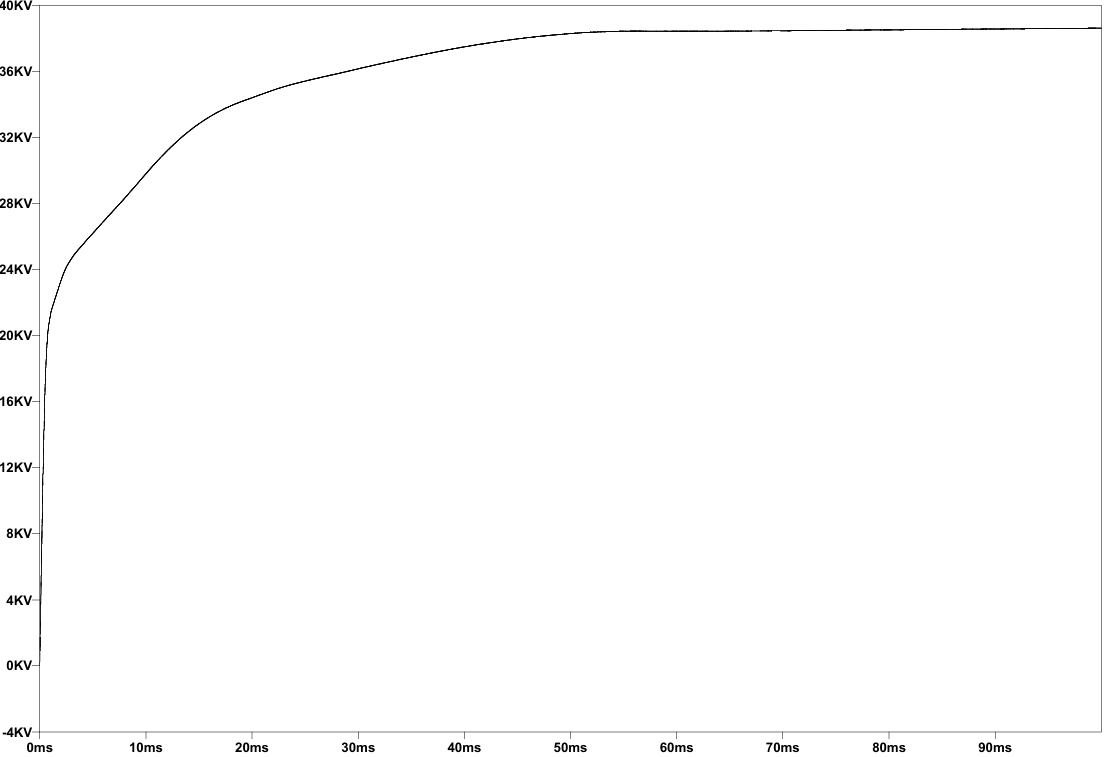
\includegraphics[width=1\textwidth]{./picture-files/cocksimu.png}}
 \caption{Simulation result of cockroft walton multiplier}
    \label{fig:simucockroft}
\end{figure}\hfill

\section{Discussion}
The simulation results confirm that the UCC21330 gate driver effectively controls both half-bridge and full-bridge configurations, producing well-defined switching waveforms with correct timing relationships and sufficient drive strength for the intended load.\\In addition, the transformer simulation verifies proper voltage step-up operation with stable waveform behavior and efficient energy transfer, indicating reliable performance under the given conditions.\\The voltage multiplier simulation further demonstrates successful voltage boosting, with stage-wise voltage buildup matching theoretical expectations and maintaining acceptable ripple levels.
\\Overall, the coordinated performance of the gate driver, transformer, and multiplier circuits validates the design approach, providing strong confidence to proceed with experimental validation on PCB prototypes.
